\documentclass{beamer}

\usetheme{simple}

\usepackage{lmodern}
\usepackage{tabularx}
\usepackage{amssymb}% http://ctan.org/pkg/amssymb
\usepackage{pifont}

% short cut for tick and cross commands
\newcommand{\yes}{\checkmark}
\newcommand{\no}{\hspace{1pt}\ding{55}}

\usepackage[scale=2]{ccicons}

%\setwatermark{\includegraphics[height=1.3cm]{img/watermark.jpg}}

\newcommand\pro{\item[\textbf{+}]}
\newcommand\con{\item[\textbf{--}]}

\title{Music synthesis with FPGAs \\and open-source tools}
\subtitle{}
\author{\texttt{github.com/schnommus/eurorack-pmod}}
\institute{Sebastian Holzapfel}
\date{}
\titlegraphic{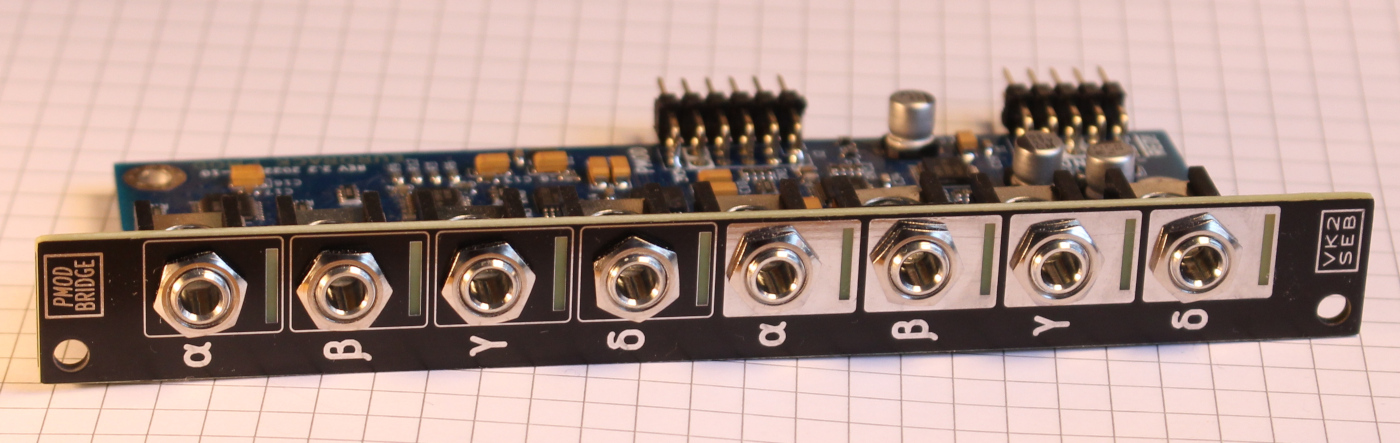
\includegraphics[height=3cm]{img/eurorack-pmod.jpg}}

\begin{document}

\maketitle

\setwatermark{}

\begin{frame}{Outline}

    \begin{itemize}
        \item Item A
        \item Preliminary work \& demo
    \end{itemize}

    \begin{block}{Mechanisms for:}
        \begin{itemize}
            \item FPGAs
            \item Synthesis
        \end{itemize}
    \end{block}

\end{frame}

% Example comment

\end{document}
